%%%%%%%%%%%%%%%%%%%%%%% file template.tex %%%%%%%%%%%%%%%%%%%%%%%%%
%
% This is a general template file for the LaTeX package SVJour3
% for Springer journals.          Springer Heidelberg 2010/09/16
%
% Copy it to a new file with a new name and use it as the basis
% for your article. Delete % signs as needed.
%
% This template includes a few options for different layouts and
% content for various journals. Please consult a previous issue of
% your journal as needed.
%
%%%%%%%%%%%%%%%%%%%%%%%%%%%%%%%%%%%%%%%%%%%%%%%%%%%%%%%%%%%%%%%%%%%
%
% First comes an example EPS file -- just ignore it and
% proceed on the \documentclass line
% your LaTeX will extract the file if required
%\begin{filecontents*}{example.eps}
%!PS-Adobe-3.0 EPSF-3.0
%%BoundingBox: 19 19 221 221
%%CreationDate: Mon Sep 29 1997
%%Creator: programmed by hand (JK)
%%EndComments
%gsave
%newpath
%  20 20 moveto
%  20 220 lineto
%  220 220 lineto
%  220 20 lineto
%closepath
%2 setlinewidth
%gsave
%  .4 setgray fill
%grestore
%stroke
%grestore
%\end{filecontents*}
%
\RequirePackage{fix-cm}
%
%\documentclass{svjour3}                     % onecolumn (standard format)
%\documentclass[smallcondensed]{svjour3}     % onecolumn (ditto)
\documentclass[smallextended]{svjour3}       % onecolumn (second format)
%\documentclass[twocolumn]{svjour3}          % twocolumn
%
\smartqed  % flush right qed marks, e.g. at end of proof
%
\usepackage{graphicx}
%
% \usepackage{mathptmx}      % use Times fonts if available on your TeX system
%
% insert here the call for the packages your document requires
%\usepackage{latexsym}
% etc.
%
% please place your own definitions here and don't use \def but
% \newcommand{}{}
%
% Insert the name of "your journal" with
% \journalname{myjournal}
%



%%%%%%%%%%%%%%%%%%%%%%
%% User-defined packages
%%%%%%%%%%%%%%%%%%%%%%

\usepackage{natbib}






%%%%%%%%%%%%%%%%%%%%%%%
\begin{document}

\title{Quantifying Interdisciplinarity of a Generalist Journal
%Indirect Bibliometrics by Hypernetwork Analysis%\thanks{Grants or other notes
%about the article that should go on the front page should be
%placed here. General acknowledgments should be placed at the end of the article.}
}
%\subtitle{Do you have a subtitle?\\ If so, write it here}

\titlerunning{Quantifying Interdisciplinarity}        % if too long for running head

\author{Juste Raimbault$^{1,2}$}

\authorrunning{J. Raimbault} % if too long for running head

\institute{J. Raimbault \at
              $^1$ UMR CNRS 8504 G{\'e}ographie-cit{\'e}s  \\
              $^2$ UMR-T IFSTTAR 9403 LVMT \\
              %Tel.: +123-45-678910\\
              %Fax: +123-45-678910\\
              \email{juste.raimbault@polytechnique.edu}           %  \\
}

\date{Received: date / Accepted: date}
% The correct dates will be entered by the editor



\maketitle

\begin{abstract}
%Insert your abstract here. Include keywords, PACS and mathematical subject classification numbers as needed.
\keywords{Bibliometrics \and Semantic Analysis}
% \PACS{PACS code1 \and PACS code2 \and more}
% \subclass{MSC code1 \and MSC code2 \and more}
\end{abstract}

%%%%%%%%%%%%%%%%%%%%%%%
\section*{Introduction}
\label{sec:intro}
%%%%%%%%%%%%%%%%%%%%%%%

Most of scientific disciplines seem to be in a need of more interdisciplinarity and transversal approaches, as explored in a recent special issue of Nature~\cite{} % TODO cite Nature special issue
, for diverse reasons that may include the development of vertically integrated fields conjointly with horizontal transversal questions~\cite{2009arXiv0907.2221B}. There are naturally ongoing debates on what is exactly interdisciplinarity (many other terms such as transdisciplinarity, crossdisciplinarity also exist) and it actually depends of involved domains : recent hybrid disciplines (see e.g. )% examples from Sanders' book
are a good illustration of the case where entanglement is strong and new discoveries are vertically deep, whereas % urbanism as a field ; 
more loose fields such as ``urbanism'' which has no precise definition and integration is by essence horizontal is an other illustration of how transversal knowledge can be produced (leading to misunderstandings when recently introduced to non-aware physicists~\cite{dupuy2015sciences}).
% ultra advanced physics : interdisciplinarity very strict ?
The question is naturally transferred into scientific communication : what are corresponding alternatives for an efficient dissemination of knowledge ? Elements of answer to such a high-level issue imply, in an evidence-based perspective, quantitative measures of interdisciplinarity.

% ``On the uncertainty of interdisciplinarity measurements due to incomplete bibliographic data'' (Scientometrics paper in Biblio)
%  -> check biblio on interdisciplinarity
%  -> the initial measurement pb

% cit Elisa's paper


The possible methods for quantitative insights into epistemology are numerous. %Existing works in quantitative epistemology using various types of networks have shown interesting potentialities.
 Using citation network features, a good predicting power for citation patterns is for example obtained by~\cite{2013arXiv1310.8220N}. Co-authorship networks can also be used for predictive models~\cite{2014arXiv1402.7268S}. A multilayer network approach was recently proposed in~\cite{2016arXiv160106075O}, using bipartites networks of papers and scholars, in order to produce measures of interdisciplinarity. Disciplines can be stratified into layers to reveal communities between them and therein collaboration patterns~\cite{2015arXiv150601280B}. Keyword networks are used in other fields such as economics of technology : for example, \cite{choi2014patent} proposes a method to identify technological opportunities by detecting important keywords from the point of view of topological measures. \cite{shibata2008detecting} uses topological analysis of the citation network to detect emerging research fronts.

We describe here a study implementing these ideas for the particular case of a scientific journal for which bibliographical data is difficult to obtain, namely \textit{Cybergeo}, an electronic journal in theoretical and quantitative geography. It makes a particularly interesting case study as deliberately generalist and concerned with open science issues such as peer-review ethics transparency~\cite{10.1371/journal.pone.0147913}, data and model practices, etc. Our approach combine semantic communities analysis (as done in~\cite{2016arXiv160208451P} for papers in physics but with keyword extraction ; \cite{2015arXiv151003797G} analyses semantic networks of political debates) with citation network to extract e.g. interdisciplinarity measures.


% TODO explain that part of a larger project ; in discussion evoke CybNetworks and the future of publishing/bibliometrics ?




% This research question is shitty, find a more relevant one
% \textbf{Research question : }\textit{How does the combination of a citation network approach with a semantic analysis unveil disciplinary context of the journal ?}



The rest of the paper is organized as follows : we describe in section~\ref{sec:data} the context of the dataset, in particular the scientific purpose of the case study journal, and the data collection procedure. We then give in section~\ref{sec:results} results on interdisciplinarity landscape obtained through network multilayer analysis of the dataset.






%Semantic analysis does not contain all the information on disciplinary compartmentation nor on patterns of propagation of scientific knowledge as the ones contained in citation networks for example. Furthermore, data collection in the previous algorithm is subject to convergence towards self-consistent themes because of the proper structure of the method. It may give more insight about scientific social patterns of ontological choices in modeling to study communities in broader networks, that would more correspond to disciplines (or sub-disciplines depending on granularity level).




%%%%%%%%%%%%%%%%%%%%%%%
\section*{Database Construction}
\label{sec:data}
%%%%%%%%%%%%%%%%%%%%%%%



%%%%%%%%%%%%%%%%%%%%%%%
%\subsection{Implementation}


The general architecture for data collection is presented in Fig.~\ref{fig:quantepistemo:data}.



\paragraph{Initial Corpus}

The production database of \textit{Cybergeo} (snapshot dump taken at date), provided by the editorial board, provides after pre-processing the initial database of articles, with basic information (title, abstract, publication year, xxx). The processed version used is available together with the full database constructed, as a \texttt{mysql} dump, at \texttt{}.



\paragraph{Citation Data}
Citation data is collected from \texttt{Google Scholar}, that is the only source for incoming citations~\cite{noruzi2005google} in our case as the journal is not referenced in other databases. We are aware of the possible biaises using this single source~\cite{bohannon2014scientific}\footnote{or see \texttt{http:\/\/iscpif.fr\/blog\/2016\/02\/the-strange-arithmetic-of-google-scholars}}, but these critics are more directed towards search results than citation counts. 


\paragraph{Text Data}

% detail mendeley collection

Text processing is done the same way as in previous section, expect that a particular treatment is done to language detection using \emph{stop-words} and a specific tagger \texttt{TreeTagger} is used for other languages than english~\cite{schmid1994probabilistic}.


%%%%%%%%%%%%%%%%%%
\begin{figure}
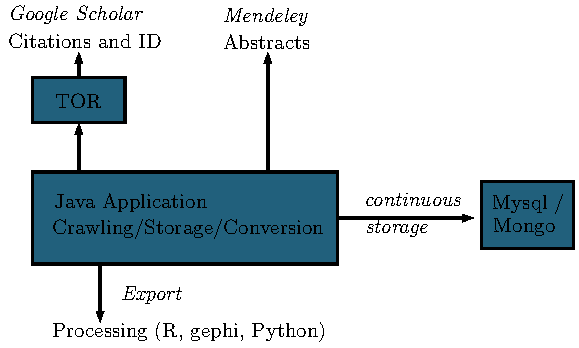
\includegraphics[width=\textwidth]{figures/archi}
\caption[Heterogeneous Bibliographical Data Collection]{Heterogeneous Bibliographical Data Collection. Architecture of the application for content (semantic data), metadata and citation data collection. The heterogeneity of tasks requires a multi-lingual approach. Source code and more precise informations on architecture are available on the \texttt{git} repository of the project at \texttt{}.}
\label{fig:datacollection}
\end{figure}
%%%%%%%%%%%%%%%%%%




%%%%%%%%%%%%%%%%%%
\begin{figure}
\centering
\includegraphics[width=0.6\textwidth]{figures/citnw}
\caption{Structure and content of the citation network. The original corpus of \emph{Cybergeo} consists in 927 articles, themselves cited by a slightly larger corpus (yielding a stationary impact factor of around 3.18), cite $\simeq 6600$ references, themselves co-cited by more than $2\cdot 10^6$ works.}
\label{fig:citationnetwork}
\end{figure}
%%%%%%%%%%%%%%%%%%









%%%%%%%%%%%%%%%%%%
\section{Methods and Results}
\label{sec:results}
%%%%%%%%%%%%%%%%%%



%%%%%%%%%%%%%%%%%%
\subsection{Citation Network Properties}


% summary stats : should be in data description ?
We are able by the reconstruction of the citation network at depth $\pm 1$ from the original 1000 references of the journal to retrieve around $45\cdot 10^6$ references, on which $2.1\cdot 10^6$ are retrieved with abstract text allowing semantic analysis. 




%%%%%%%%%%%%%%%%%
\begin{figure}
\centering
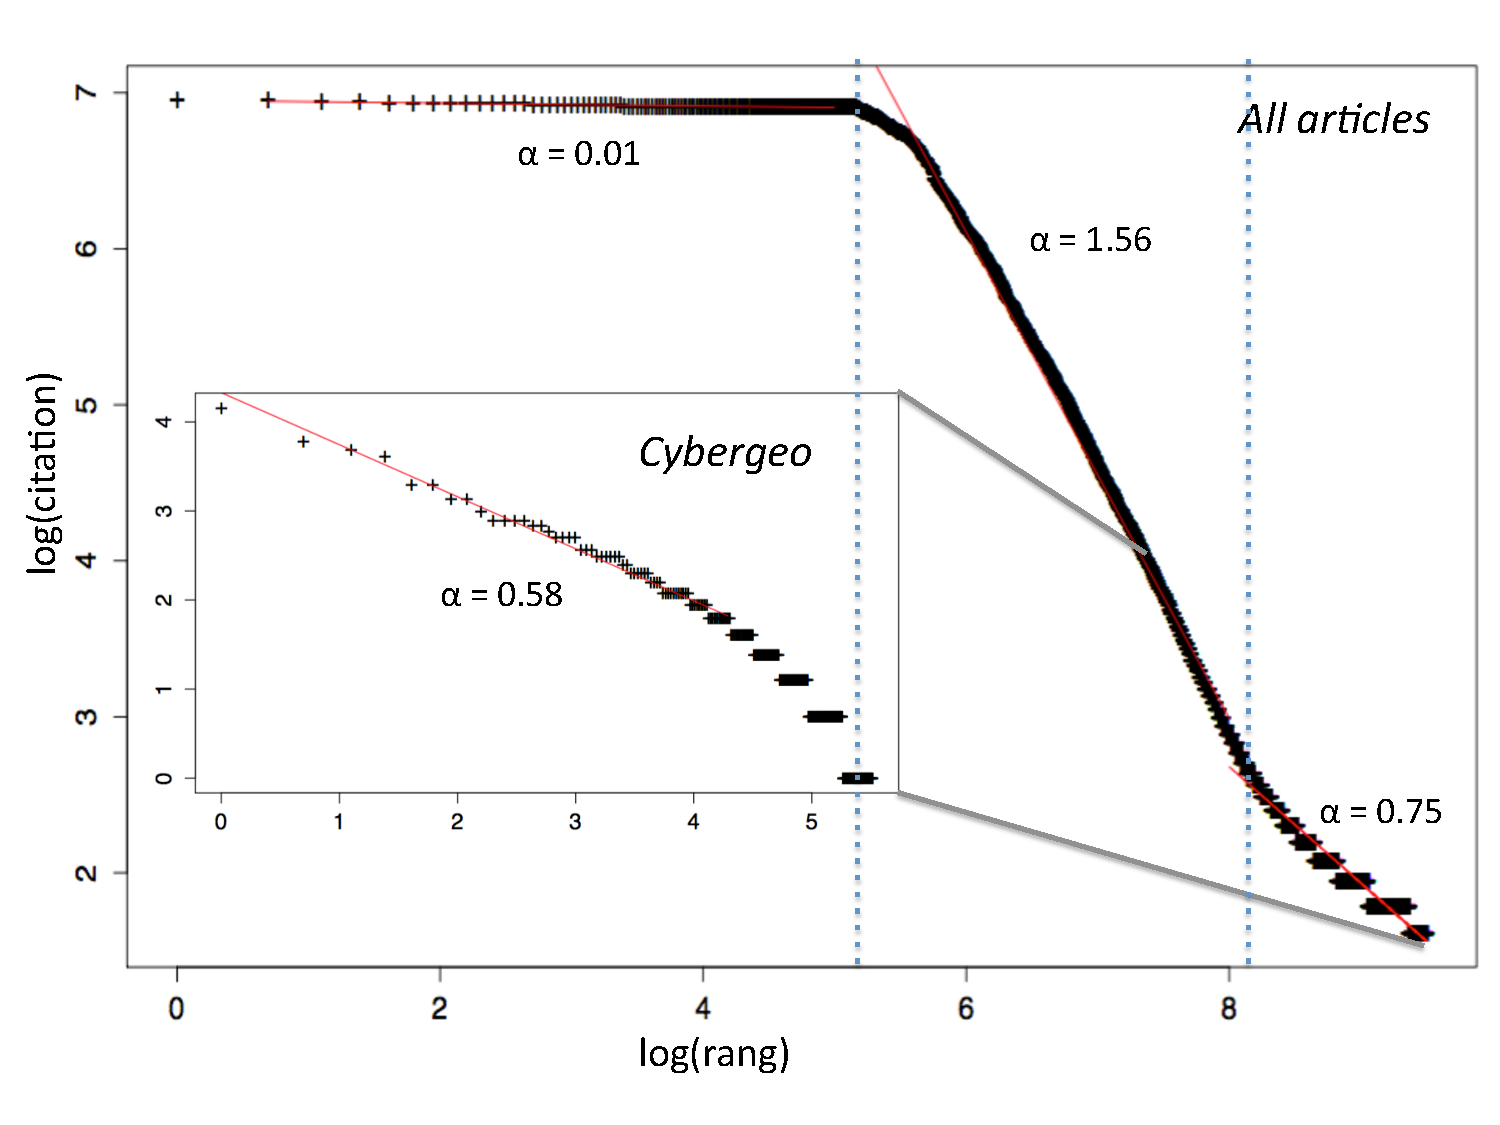
\includegraphics[width=0.8\textwidth]{figures/ranksize.pdf}
\caption[Properties of the citation network]{Properties of the citation network. Rank-size plot of in-degrees ; three superposing successive regimes must correspond to different literature types or practices across disciplines.}
\label{fig:quantepistemo:citnw}
\end{figure}
%%%%%%%%%%%%%%%%%


%%%%%%%%%%%%%%%%%
\begin{figure}
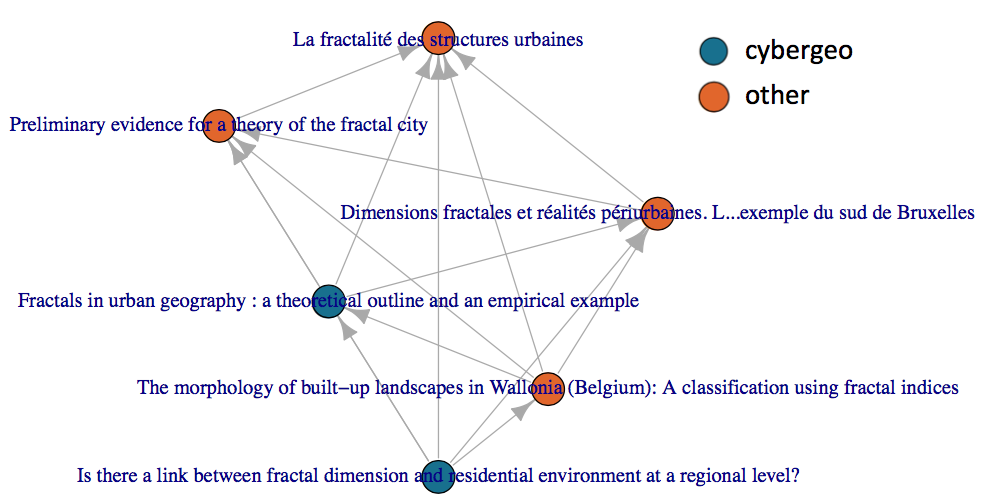
\includegraphics[width=\textwidth]{figures/cybclic.png}
\caption[Example of clique in the citation network]{Example of a maximal clique in the citation network, paper of \texttt{cybergeo} being in blue. Such topological structure reveal citation practices such as here a systematic citation of previous works in the research niche.}
\label{fig:quantepistemo:cliques}
\end{figure}
%%%%%%%%%%%%%%%%%



%%%%%%%%%%%%%%%%%%
\subsection{Semantic Communities Construction}



%%%%%%%%%%%%%%%%%%
\paragraph{Relevant Keywords Extraction}


\textit{Text-mining in python with \texttt{nltk}~\cite{bird2006nltk}}, method adpated from
\cite{chavalarias2013phylomemetic}


\bigskip

\begin{itemize}
\item Language detection using \textit{stop-words}
\item Parsing and tokenizing / pos-tagging (word functions) / stemming done differently depending on language :
\begin{itemize}
\item English : \texttt{nltk} built-in pos-tagger, combined to a \emph{PorterStemmer}
\item French or other : use of \texttt{TreeTagger}~\cite{schmid1994probabilistic}
\end{itemize}
\item Selection of potential \textit{n-grams} (with $1 \leq n \leq 4$) : English $\bigcap \{NN \cup VBG \cup JJ \}$ ;  French  $\bigcap \{NOM \cup ADJ\}$
\item Database insertion for instantaneous utilisation (10j $\rightarrow$ 2min)
\item Estimation of \textit{n-grams} relevance, following co-occurrences statistical distribution
\end{itemize}



%%%%%%%%%%%%%%%%%%
\paragraph{Semantic Network}

% describe co-occurrence nw








%%%%%%%%%%%%%%%%%%
\begin{figure}
\hspace{-2cm}
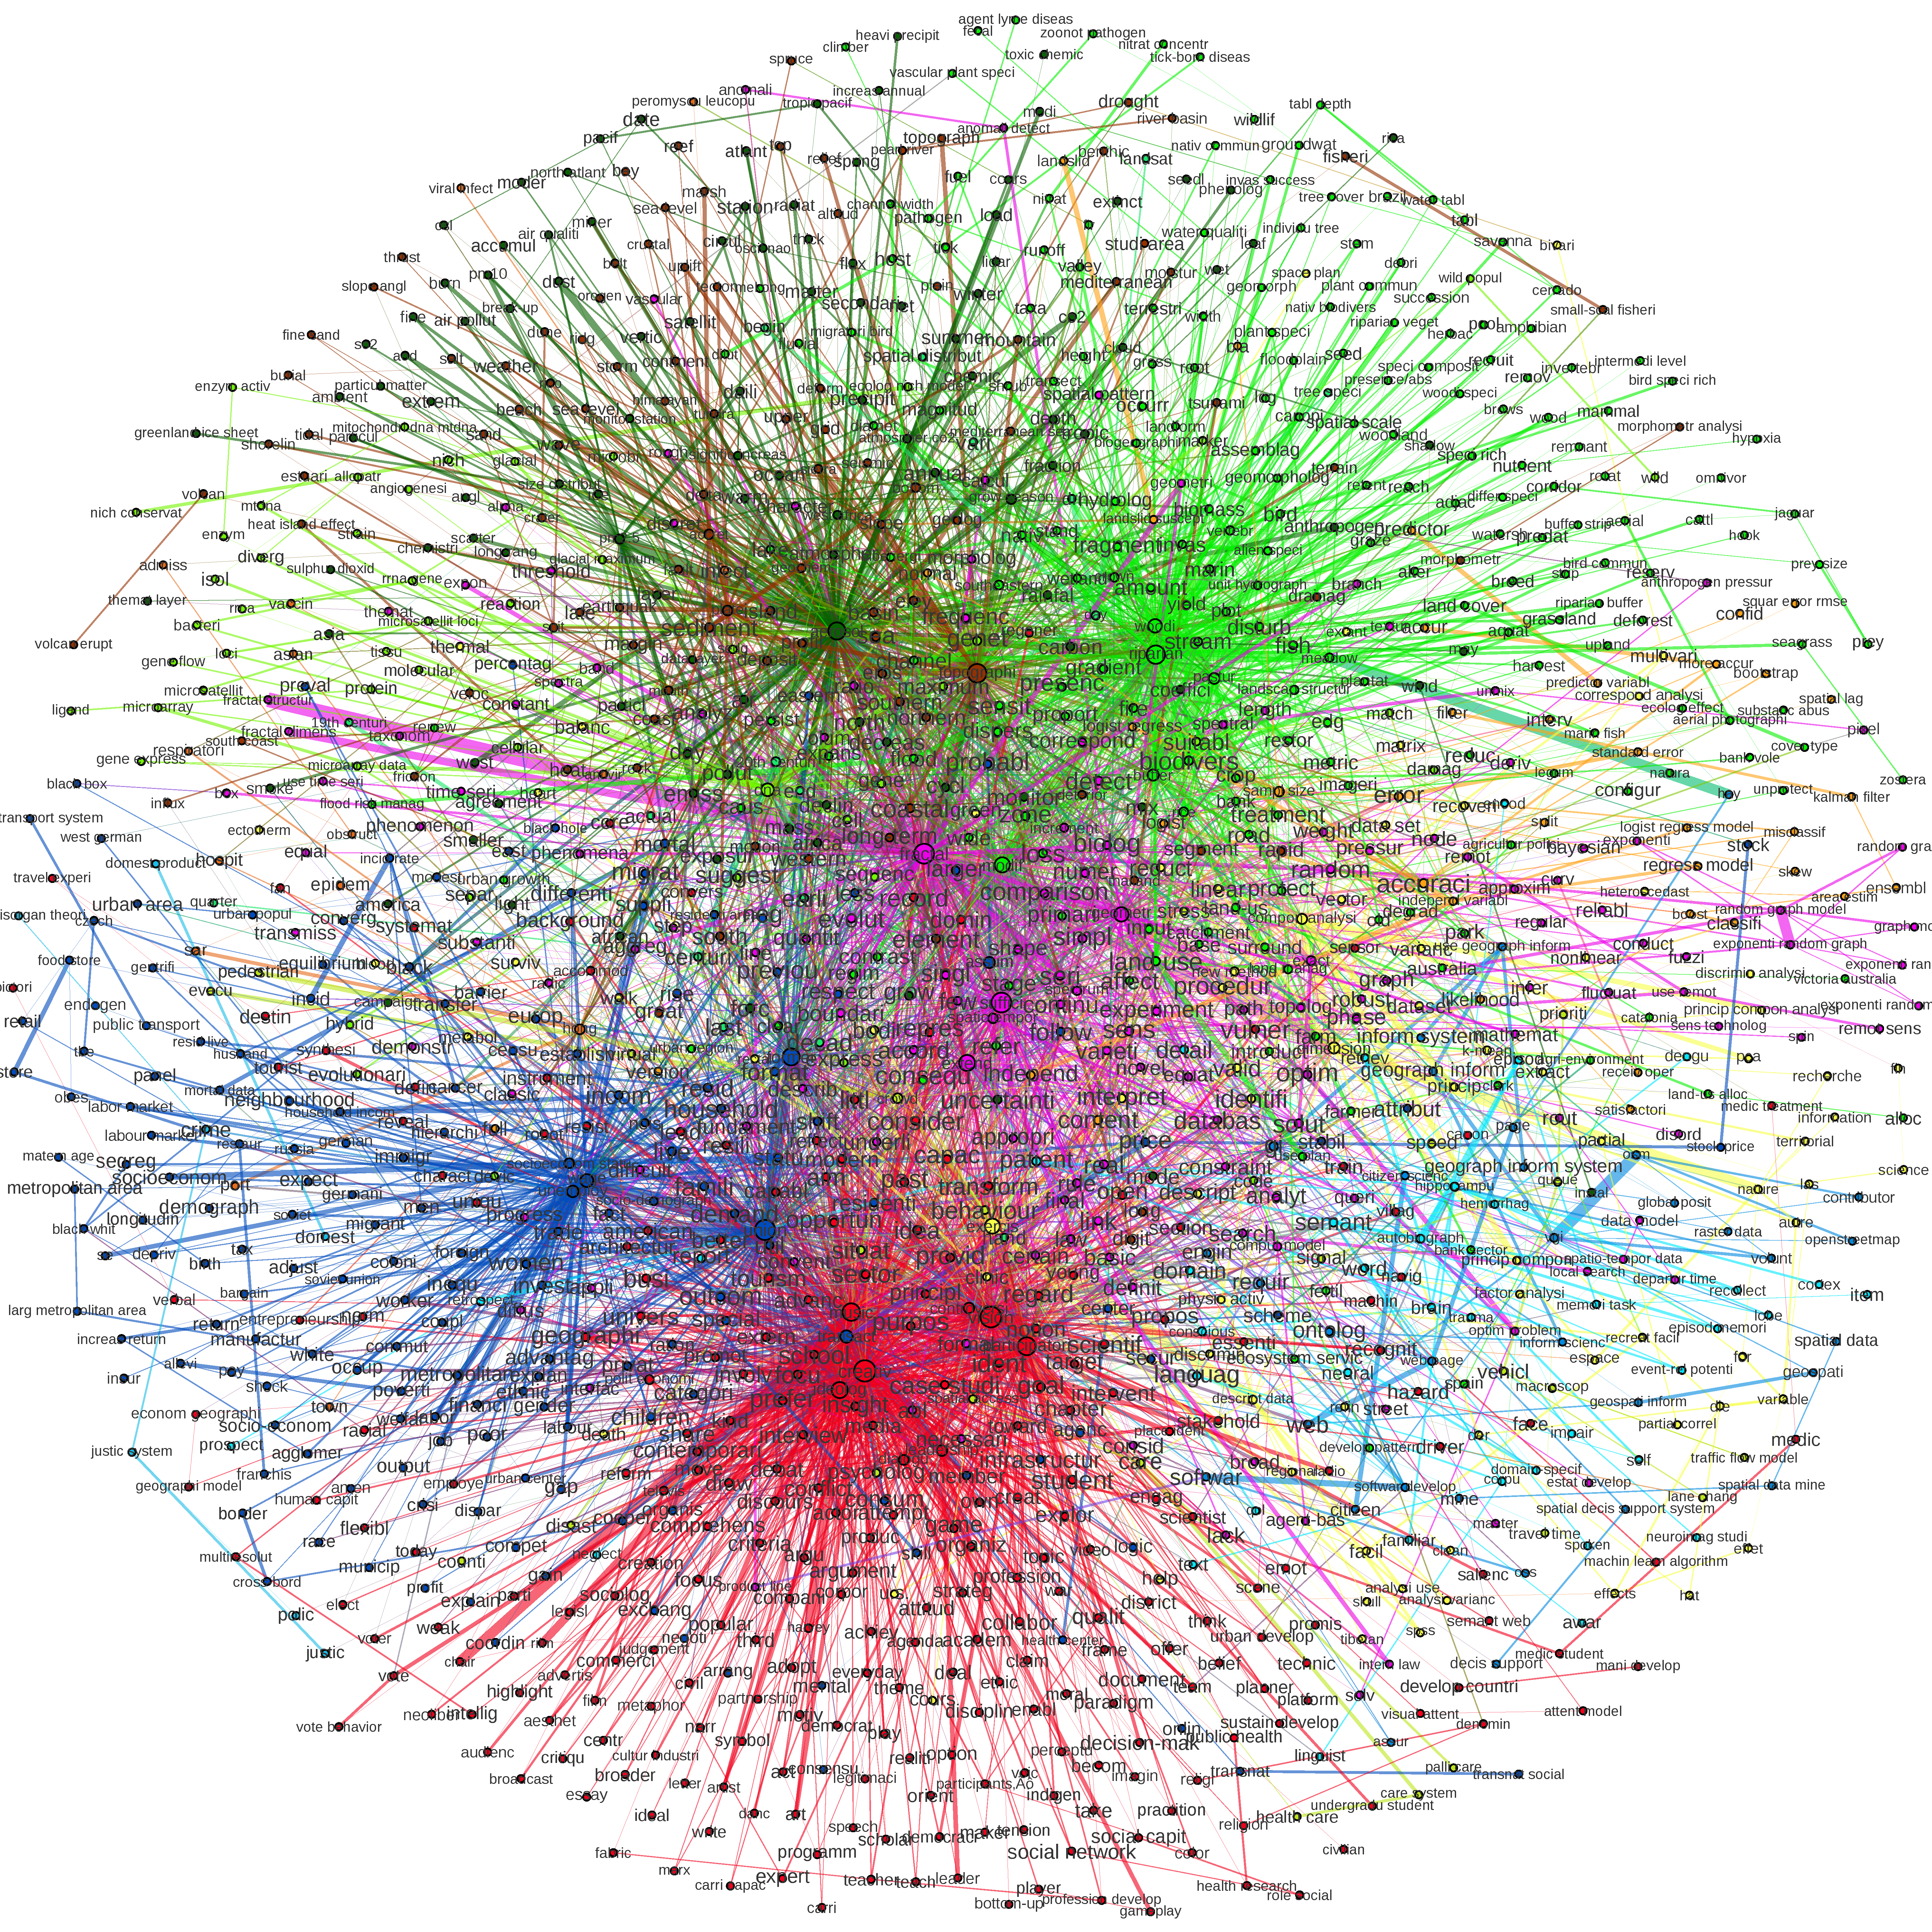
\includegraphics[width=1.6\textwidth]{figures/semantic.png}
\caption[Semantic network of concepts in quantitative geography]{Semantic network of concepts in quantitative geography. Corpus consists of around $2\cdot 10^5$ abstracts of publications at a topological distance shorter than 2 from the journal \texttt{cybergeo} in the citation network. Relevance of keywords were estimated with a bootstrap method, and semantic network is constructed by co-occurrences of keywords (filtered following the procedure detailed in text, with cut at larger degrees of 10\% here to delete hubs such as \texttt{model} or \texttt{space} and efficiently reveal communities). A zoomable vectorial file (\texttt{.svg}) of the network is available as Supplementary Material.}
\label{fig:quantepistemo:semanticnw}
\end{figure}
%%%%%%%%%%%%%%%%%%




%%%%%%%%%%%%%%%%%%
\paragraph{Sensitivity Analysis}


% sensitivity analysis to params/meta-params






%%%%%%%%%%%%%%%%%%
\paragraph{Communities}

We retrieve by community detection in the semantic network typical geographical disciplines, such as :

\begin{itemize}
\item Political sciences/critical geography (535) : \texttt{decision-mak, polit ideolog, democraci, stakehold, neoliber}
\item Biogeography (394) : \texttt{plant densiti, wood, wetland, riparian veget}
\item Economic geography (343) : \texttt{popul growth, transact cost, socio-econom, household incom}
\item Environnment/climate (309) : \texttt{ice sheet, stratospher, air pollut, climat model}
\item Complex systems (283) : \texttt{scale-fre, multifract, agent-bas model, self-organ}
\item Physical geography (203) : \texttt{sedimentari, digit elev model, geolog, river delta}
\item Spatial analysis (175) : \texttt{spatial analysi, princip compon analysi, heteroscedast, factor analysi}
\item Microbiology (118) : \texttt{chromosom, phylogenet, borrelia}
\item Statistical methods (88) : \texttt{logist regress, classifi, kalman filter, sampl size}
\item Cognitive sciences (81) : \texttt{semant memori, retrospect, neuroimag}
\item GIS (75) : \texttt{geograph inform scienc, softwar design, volunt geograph inform, spatial decis support}
\item Traffic modeling (63) : \texttt{simul model, lane chang, traffic flow, crowd behavior}
\item Health (52) : \texttt{epidem, vaccin strategi, acut respiratori syndrom, hospit}
\item Remote sensing (48) : \texttt{land-cov, landsat imag, lulc}
\item Crime (17) : \texttt{crimin justic system, social disorgan, crime}
\end{itemize}





%%%%%%%%%%%%%%%%%%
\subsection{Measures of Interdisciplinarity}





Distribution of keywords within reconstructed disciplines provides an article-level interdisciplinarity, and we can construct various measures at the journal level. Combination of citation and semantic layers in the hyper-network provide second order interdisciplinarity measures. The construction of null models for comparison and the collection of currently missing data (journals for other papers) are currently ongoing so these results are not presented here.














%%%%%%%%%%%%%%%%%%
\section{Discussion}
\label{sec:discussion}
%%%%%%%%%%%%%%%%%%










%%%%%%%%%%%%%%%%%%
\section{Conclusion}
\label{sec:discussion}
%%%%%%%%%%%%%%%%%%












%%%%%%%%%%%%%%%%%%%%%
%%%%%%%%%%%%%%%%%%%%%

\begin{acknowledgements}
The author would like to thank the editorial board of Cybergeo, and more particularly Denise Pumain, for having offered the opportunity to work on that subject and provided the production database of the journal. 
\end{acknowledgements}





%%%%%%%%%%%%%%%%%%%%%
% Biblio
%%%%%%%%%%%%%%%%%%%%%


% BibTeX users please use one of
\bibliographystyle{spbasic}      % basic style, author-year citations
\bibliography{biblio}   % name your BibTeX data base













%%%%%%%%%%%%%%%%%%%%%
%%   Templates
%%%%%%%%%%%%%%%%%%%%%


%
%% For one-column wide figures use
%\begin{figure}
%% Use the relevant command to insert your figure file.
%% For example, with the graphicx package use
%  \includegraphics{example.eps}
%% figure caption is below the figure
%\caption{Please write your figure caption here}
%\label{fig:1}       % Give a unique label
%\end{figure}
%%
%% For two-column wide figures use
%\begin{figure*}
%% Use the relevant command to insert your figure file.
%% For example, with the graphicx package use
%  \includegraphics[width=0.75\textwidth]{example.eps}
%% figure caption is below the figure
%\caption{Please write your figure caption here}
%\label{fig:2}       % Give a unique label
%\end{figure*}
%%
%% For tables use
%\begin{table}
%% table caption is above the table
%\caption{Please write your table caption here}
%\label{tab:1}       % Give a unique label
%% For LaTeX tables use
%\begin{tabular}{lll}
%\hline\noalign{\smallskip}
%first & second & third  \\
%\noalign{\smallskip}\hline\noalign{\smallskip}
%number & number & number \\
%number & number & number \\
%\noalign{\smallskip}\hline
%\end{tabular}
%\end{table}
%











\end{document}
% end of file template.tex

